\documentclass[11pt,a4paper]{article}
\usepackage[T1]{fontenc}
\usepackage[utf8]{inputenc}
\usepackage[english]{babel}
\usepackage{geometry,xcolor,array,booktabs,longtable,tabularx,tikz,fancyhdr,titlesec,enumitem,hyperref,lastpage,microtype}
\usepackage[sfdefault]{noto}
\usepackage[most]{tcolorbox}
\usepackage{pdflscape}
\usetikzlibrary{arrows.meta,calc,positioning,shapes.geometric,babel}

\geometry{left=18mm,right=18mm,top=21mm,bottom=20mm,headheight=20pt}
\setlength{\parindent}{0pt}
\setlength{\parskip}{5pt}
\setlength{\emergencystretch}{2em}
\setlist{nosep,leftmargin=*}
\definecolor{limblue}{HTML}{102A43}
\definecolor{limcyan}{HTML}{00A6A6}
\definecolor{limaccent}{HTML}{FF6B4A}
\definecolor{limmint}{HTML}{DFF7F5}
\definecolor{limlight}{HTML}{F1F5F8}
\definecolor{limpaper}{HTML}{FAFCFD}
\definecolor{limgray}{HTML}{627D98}
\hypersetup{colorlinks=true,linkcolor=limcyan,urlcolor=limcyan,pdftitle={LIM M2 --- Processor Architecture Reference Manual}}
\pagestyle{fancy}
\fancyhf{}
\fancyhead[L]{\colorbox{limblue}{\textcolor{white}{\strut\hspace{2mm}\textbf{LIM M2}\hspace{2mm}}}}
\fancyhead[R]{\small\textcolor{limgray}{PROCESSOR REFERENCE MANUAL / REVISION 0.2}}
\fancyfoot[L]{\small LIM M2 Reference Manual --- Revision 0.2 (October 2026)}
\fancyfoot[R]{\small \thepage/\pageref{LastPage}}
\renewcommand{\headrulewidth}{0pt}
\renewcommand{\footrulewidth}{0pt}
\titleformat{\section}{\Large\bfseries\color{limblue}}
  {\colorbox{limcyan}{\textcolor{white}{\strut\thesection}}}{0.75em}{}
\titleformat{\subsection}{\large\bfseries\color{limblue}}{\thesubsection}{0.7em}{}
\titlespacing*{\section}{0pt}{16pt}{8pt}

\newcommand{\TBD}{\textcolor{limcyan}{\textbf{TBD}}}
\newcommand{\reg}[1]{\texttt{#1}}
\newcommand{\bits}[1]{\texttt{#1}}
\newcommand{\field}[1]{\textsf{#1}}
\newcommand{\opcodebox}[1]{\tikz[baseline=(n.base)]\node[fill=limblue,text=white,rounded corners=2pt,inner xsep=7pt,inner ysep=3pt,font=\ttfamily\bfseries] (n) {#1};}
\newtcolorbox{limnote}[1]{
  enhanced,breakable,colback=limlight,colframe=limcyan,boxrule=0pt,
  borderline west={3pt}{0pt}{limcyan},arc=1mm,left=4mm,right=4mm,
  top=3mm,bottom=3mm,title={#1},fonttitle=\bfseries\color{limblue},
  coltitle=limblue,attach title to upper={\par\smallskip}}
\newtcolorbox{specbox}{
  enhanced,colback=limpaper,colframe=limlight,boxrule=0.8pt,arc=2mm,
  left=3mm,right=3mm,top=2mm,bottom=2mm}

\newcommand{\InstructionPage}[8]{%
  \clearpage
  \phantomsection\addcontentsline{toc}{subsection}{#1 --- #4}
  \begin{tcolorbox}[enhanced,colback=limblue,colframe=limblue,arc=3mm,
    left=5mm,right=5mm,top=4mm,bottom=4mm]
  \begin{minipage}[t]{0.68\textwidth}
    {\fontsize{30}{34}\selectfont\bfseries\color{white}#1}\par\vspace{1mm}
    {\large\color{white}#4}
  \end{minipage}\hfill
  \begin{minipage}[t]{0.25\textwidth}\raggedleft
    \tikz[baseline=(n.base)]\node[fill=limcyan,text=white,rounded corners=2pt,
      inner xsep=8pt,inner ysep=4pt,font=\ttfamily\bfseries] (n) {#2};
    \par\smallskip{\small\color{white}#3}
  \end{minipage}
  \end{tcolorbox}
  \vspace{3mm}
  \begin{specbox}
  \begin{tabularx}{\dimexpr\textwidth-8mm\relax}{>{\bfseries\color{limblue}}p{31mm}X}
    \toprule
    Mnemonic & \texttt{#1} \\
    Opcode & \bits{#2} (Upper 5 bits of instruction word) \\
    Encoding & 5-bit opcode, 3-bit \field{cfg} field, followed by dynamic arguments (direct arguments for specialized commands) \\
    Class & #3 \\
    Status & Core specification ratified; argument bitfields and extended options undergoing final layout \\
    \bottomrule
  \end{tabularx}
  \end{specbox}
  \subsection*{Instruction Purpose} #4.
  \subsection*{Architectural Semantics}
  \begin{tcolorbox}[colback=limmint,colframe=limmint,arc=2mm,boxrule=0pt,left=4mm]
    \ttfamily #5
  \end{tcolorbox}
  \subsection*{Configuration and Operands} #6
  \subsection*{Flags Affected (FREG)} #7
  \subsection*{Datapath Micro-Operations}
  \begin{enumerate}
    \item Multiplexer selection of source operands from register file or immediate bus.
    \item Operation dispatch to dedicated execution block (ALU / memory / control).
    \item Result routing via Writeback selector (MUX 2) to destination register with write-enable gating.
    \item Synchronous status update of \reg{FREG} and pointer registers (\reg{PTREG}, \reg{SREG}).
  \end{enumerate}
  Cycle breakdown and control strobes: \TBD.
  \subsection*{Implementation Notes} #8
  \vfill{\footnotesize\color{limgray}TBD markers denote configurable hardware options.}
}

\begin{document}
\begin{titlepage}
  \pagecolor{limpaper}\color{limblue}
  \begin{tikzpicture}[remember picture,overlay]
    \fill[limblue] (current page.north west) rectangle
      ([xshift=58mm]current page.south west);
    \fill[limcyan] ([xshift=58mm]current page.north west) rectangle
      ([xshift=63mm]current page.south west);
    \draw[limlight,line width=0.7pt] ([xshift=77mm,yshift=-37mm]current page.north west)
      -- ([xshift=-16mm,yshift=-37mm]current page.north east);
  \end{tikzpicture}
  \vspace*{18mm}
  \hspace*{-7mm}\begin{minipage}{50mm}\centering
    {\color{white}\bfseries\large HIGH-PERFORMANCE}\par\smallskip
    {\color{limcyan}\bfseries\small 16-BIT ARCHITECTURE}
  \end{minipage}\par
  \vspace{31mm}
  \hspace*{68mm}\begin{minipage}{100mm}\raggedright
    {\fontsize{38}{42}\selectfont\bfseries LIM\par M2}\par
    \vspace{7mm}
    {\Large\bfseries\color{limcyan}Processor Architecture Reference Manual}\par
    \vspace{9mm}
    {\large A deterministic, high-frequency 16-bit microprogrammed processor architecture featuring conflict-free multiplexer routing and 24-bit extended addressing.}\par
    \vspace{18mm}
    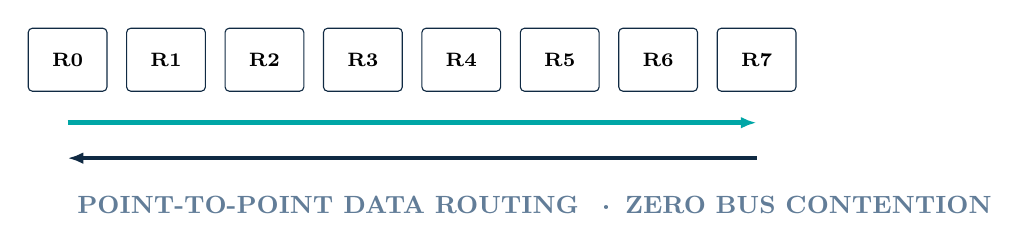
\begin{tikzpicture}[node distance=5mm]
      \foreach \x/\n in {0/R0,1.25/R1,2.5/R2,3.75/R3,5/R4,6.25/R5,7.5/R6,8.75/R7}
        \node[draw=limblue,rounded corners=1.5pt,minimum width=10mm,minimum height=8mm,
          fill=white,font=\bfseries\scriptsize] (r\n) at (\x,0) {\n};
      \draw[limcyan,line width=2pt,-{Latex[length=2mm]}] (0,-0.8) -- (8.75,-0.8);
      \draw[limblue,line width=1.2pt,-{Latex[length=2mm]}] (8.75,-1.25) -- (0,-1.25);
      \node[anchor=west,font=\small\bfseries,text=limgray] at (0,-1.85)
        {POINT-TO-POINT DATA ROUTING \enspace·\enspace ZERO BUS CONTENTION};
    \end{tikzpicture}
  \end{minipage}
  \vfill
  \hspace*{68mm}\begin{minipage}{100mm}\raggedright
    {\bfseries\color{limaccent}OFFICIAL REFERENCE SPECIFICATION}\par\smallskip
    {\large Revision 0.2 --- October 2026}\par\medskip
    {\small\color{limgray}LIM M2 Core Architecture Manual. All rights reserved.}
  \end{minipage}
  \vspace*{10mm}
\end{titlepage}
\nopagecolor

\tableofcontents
\clearpage

\section{Document Scope and Architectural Philosophy}
This document serves as the formal architectural reference manual and hardware specification for the \textbf{LIM M2} microprocessor. The LIM M2 architecture has been deliberately designed to deliver deterministic execution, robust electrical integrity, and superior clock scaling.

A defining cornerstone of the LIM M2 datapath is the \textbf{total elimination of internal tri-state (high-impedance / Hi-Z) buses}. By substituting shared capacitive wires with actively driven multiplexer trees (Point-to-Point MUX Routing), the architecture prevents shoot-through currents, eliminates bus contention risks, and guarantees sharp, symmetrical transition edges.

\begin{limnote}{Instruction Code Allocation}
The LIM M2 instruction set architecture utilizes a contiguous 5-bit primary opcode space:
\texttt{NOP}=0, \texttt{ADD}=1, \ldots, \texttt{CSRM}=26. Opcode values 27--31 are reserved for next-generation hardware extensions.
\end{limnote}

\subsection{Notational Conventions}
\begin{tabularx}{\textwidth}{>{\ttfamily}p{28mm}X}
\toprule
Notation & Architectural Meaning \\
\midrule
dst & Destination register targeted for writeback \\
src, srcA, srcB & Source register operand identifiers \\
imm & Immediate constant scalar embedded within the instruction \\
addr & Memory address (16-bit primary or 24-bit extended pointer) \\
cfg & 3-bit operational mode configuration field \\
ZF, CF, OF & Hardware status flags (Zero, Carry, and Overflow) within \reg{FREG} \\
\bottomrule
\end{tabularx}

\section{Processor Overview}
The \textbf{LIM M2} is a versatile, high-throughput 16-bit microprogrammed processor engineered for integer-intensive computation. Architectural highlights include:

\begin{itemize}
  \item \textbf{Conflict-Free Multiplexer Datapath:} Internal signals are steered purely by push-pull multiplexer trees (\textbf{MUX 1}, \textbf{DEST-DMUX}, and \textbf{MUX 2}). This modern design is perfectly suited for high-density ASIC and modern FPGA synthesis.
  \item \textbf{Dual Accumulator Staging:} Dedicated pre-ALU accumulators (\reg{ACCA} and \reg{ACCB}) isolate the arithmetic core from the general register file, minimizing propagation path skew.
  \item \textbf{Hardware ALU Auto-Chaining (Multi-Word Arithmetic):} The ALU integrates an internal residual register (\reg{ALU\_RESIDUAL}). When an addition overflows 16 bits ($>2^{16}-1$), a subtraction produces a borrow ($<0$), or multiplication/division produces high-word residuals, the excess is retained in hardware and automatically accumulated or subtracted in the next mathematical operation. This enables continuous multi-word arithmetic (32, 48, 64+ bits) without dedicated ADC/SBB instructions. The chain is flushed using \texttt{NOP}.
  \item \textbf{Direct Reg-to-Reg Bypass:} A low-latency path from MUX 1 directly into MUX 2 enables single-cycle register transfers without locking ALU resources.
  \item \textbf{Linear 24-Bit Addressing (Up to 16 MB):} Dedicated 24-bit pointer registers (\reg{PTREG} with auto-increment and \reg{SREG} stack pointer) transcend the traditional 64 KB memory barrier, providing linear access across 16 megabytes of data and stack space.
  \item \textbf{High Clock Scaling Potential:} Unburdened by capacitive bus decay, the LIM M2 operates comfortably at a baseline frequency of \textbf{200~MHz}, scaling toward \textbf{700~MHz and above} in optimized silicon.
\end{itemize}

\clearpage
\begin{landscape}
\thispagestyle{empty}
\subsection{Conceptual Datapath Schematic}
\begin{center}
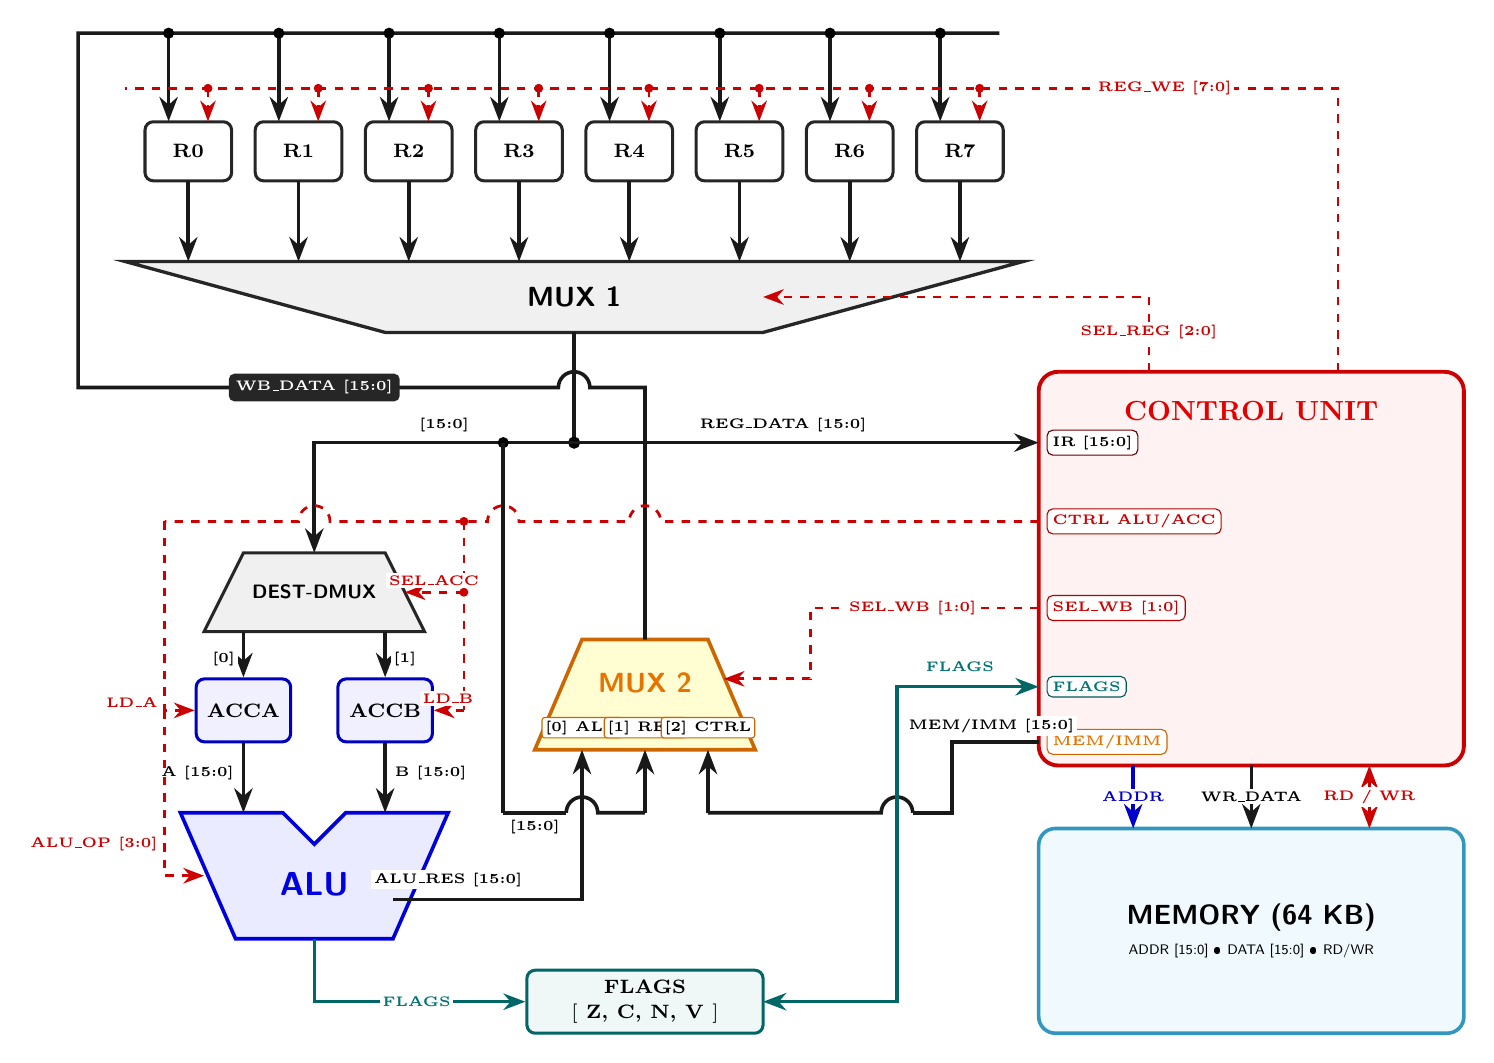
\begin{tikzpicture}[
    x=1cm, y=1cm,
    >=Stealth,
    font=\sffamily\scriptsize,
    % Component Styles
    regnode/.style={
        draw=black!85, rectangle, rounded corners=3pt, minimum width=1.1cm, minimum height=0.75cm, 
        line width=1.1pt, fill=white, font=\bfseries\scriptsize, align=center
    },
    block/.style={
        draw=black!85, rectangle, rounded corners=3pt, line width=1.1pt, fill=white, 
        font=\bfseries\scriptsize, align=center
    },
    ctrlbox/.style={
        draw=red!80!black, rectangle, rounded corners=7pt, line width=1.4pt,
        fill=red!5, align=center
    },
    membox/.style={
        draw=cyan!75!black, rectangle, rounded corners=6pt, line width=1.3pt,
        fill=cyan!6, align=center
    },
    % Wire Styles
    databus/.style={->, line width=1.3pt, draw=black!90},
    databus_line/.style={line width=1.3pt, draw=black!90},
    ctrlbus/.style={->, line width=1.0pt, draw=red!80!black, dashed},
    ctrlbus_line/.style={line width=1.0pt, draw=red!80!black, dashed},
    bidir/.style={<->, line width=1.2pt, draw=teal!80!black}
]

    % ========================================================
    % 1. РЕГИСТРЫ R0 - R7 (16-BIT GPR) (Y = 12.0)
    % ========================================================
    \foreach \i/\x in {0/0.6, 1/2.0, 2/3.4, 3/4.8, 4/6.2, 5/7.6, 6/9.0, 7/10.4} {
        \node[regnode] (R\i) at (\x, 12.0) {\textbf{R\i}};
        \coordinate (R\i_in) at (\x - 0.25, 12.38);
        \coordinate (R\i_we) at (\x + 0.25, 12.38);
        \coordinate (R\i_out) at (\x, 11.62);
    }

    % ========================================================
    % 2. MUX 1 (REG MUX) (Y = 9.7 .. 10.6, Center X = 5.5)
    % ========================================================
    \draw[fill=gray!12, draw=black!85, line width=1.2pt] 
        (-0.2, 10.6) -- (11.2, 10.6) -- (7.9, 9.7) -- (3.1, 9.7) -- cycle;
    \node[align=center] at (5.5, 10.15) {\textbf{\normalsize MUX 1}};

    % Спуски от каждого регистра в MUX 1
    \foreach \i in {0,...,7} {
        \draw[databus] (R\i_out) -- (R\i_out |- 0, 10.6);
    }

    % ========================================================
    % 3. ЛЕВАЯ КОЛОНКА: DEST-DMUX, ACCA, ACCB, ALU (16-BIT)
    % ========================================================
    % DEST-DMUX (Center X = 2.2, Y = 5.9 .. 6.9)
    \draw[fill=gray!12, draw=black!85, line width=1.1pt] 
        (1.3, 6.9) -- (3.1, 6.9) -- (3.6, 5.9) -- (0.8, 5.9) -- cycle;
    \node[align=center] at (2.2, 6.4) {\textbf{\scriptsize DEST-DMUX}};

    % Аккумуляторы ACCA и ACCB (Y = 4.9)
    \node[regnode, fill=blue!6, draw=blue!75!black, minimum width=1.2cm, minimum height=0.8cm] 
        (ACCA) at (1.3, 4.9) {\textbf{ACCA}};
    \node[regnode, fill=blue!6, draw=blue!75!black, minimum width=1.2cm, minimum height=0.8cm] 
        (ACCB) at (3.1, 4.9) {\textbf{ACCB}};

    % Связи от DMUX к аккумуляторам
    \draw[databus] (1.3, 5.9) -- (ACCA.north);
    \draw[databus] (3.1, 5.9) -- (ACCB.north);
    \node[font=\tiny\bfseries, fill=white, inner sep=1pt] at (1.05, 5.55) {[0]};
    \node[font=\tiny\bfseries, fill=white, inner sep=1pt] at (3.35, 5.55) {[1]};

    % ALU (Center X = 2.2, Y = 2.0 .. 3.6)
    \draw[fill=blue!8, draw=blue!85!black, line width=1.3pt]
        (0.5, 3.6) -- (1.8, 3.6) -- (2.2, 3.2) -- (2.6, 3.6) -- (3.9, 3.6) -- (3.2, 2.0) -- (1.2, 2.0) -- cycle;
    \node[align=center, text=blue!90!black] at (2.2, 2.7) {\textbf{\large ALU}};

    % Входы в ALU от аккумуляторов
    \draw[databus] (ACCA.south) -- (1.3, 3.6);
    \draw[databus] (ACCB.south) -- (3.1, 3.6);
    \node[font=\tiny\bfseries, left] at (1.3, 4.1) {A [15:0]};
    \node[font=\tiny\bfseries, right] at (3.1, 4.1) {B [15:0]};

    % ========================================================
    % 4. ЦЕНТРАЛЬНАЯ КОЛОНКА: MUX 2 (MEM MUX) И FLAG REG
    % ========================================================
    % MUX 2: ПЕРЕВЕРНУТ! (Узкий верх Y = 5.8, широкий низ Y = 4.4, Center X = 6.4)
    \draw[fill=yellow!18, draw=orange!80!black, line width=1.3pt]
        (5.6, 5.8) -- (7.2, 5.8) -- (7.8, 4.4) -- (5.0, 4.4) -- cycle;
    \node[align=center, text=orange!90!black] at (6.4, 5.25) {\textbf{\normalsize MUX 2}};

    % Бейджи входов MUX 2 ВНУТРИ трапеции по нижнему краю
    \node[font=\tiny\bfseries, fill=white, draw=orange!80!black, rounded corners=1pt, inner sep=1.2pt] at (5.6, 4.68) {[0] ALU};
    \node[font=\tiny\bfseries, fill=white, draw=orange!80!black, rounded corners=1pt, inner sep=1.2pt] at (6.4, 4.68) {[1] REG};
    \node[font=\tiny\bfseries, fill=white, draw=orange!80!black, rounded corners=1pt, inner sep=1.2pt] at (7.2, 4.68) {[2] CTRL};

    % Флаговый регистр (Center X = 6.4, Y = 1.2, W = 3.0cm, H = 0.8cm)
    \node[block, minimum width=3.0cm, minimum height=0.8cm, fill=teal!6, draw=teal!80!black] 
        (FLAGS) at (6.4, 1.2) {\textbf{FLAGS}\\[1pt]\scriptsize$[$ Z, C, N, V $]$};

    % ========================================================
    % 5. ПРАВАЯ КОЛОНКА: КОНТРОЛЛЕР И ПАМЯТЬ
    % ========================================================
    % Контроллер (X = 11.4 .. 16.8, Y = 4.2 .. 9.2, Center X = 14.1)
    \node[ctrlbox, minimum width=5.4cm, minimum height=5.0cm] 
        (CTRL) at (14.1, 6.7) {};
    
    % Заголовок контроллера
    \node[font=\bfseries\normalsize, text=red!90!black] at (14.1, 8.7) {CONTROL UNIT};

    % Порты на левой стенке Контроллера (X = 11.4)
    \node[draw=red!40!black, fill=white, rounded corners=2pt, font=\tiny\bfseries, inner sep=2pt, right] 
        at (11.5, 8.3) {IR [15:0]};
    \node[draw=red!70!black, fill=white, rounded corners=2pt, font=\tiny\bfseries, inner sep=2pt, text=red!80!black, right] 
        at (11.5, 7.3) {CTRL ALU/ACC};
    \node[draw=red!70!black, fill=white, rounded corners=2pt, font=\tiny\bfseries, inner sep=2pt, text=red!80!black, right] 
        at (11.5, 6.2) {SEL\_WB [1:0]};
    \node[draw=teal!70!black, fill=white, rounded corners=2pt, font=\tiny\bfseries, inner sep=2pt, text=teal!90!black, right] 
        at (11.5, 5.2) {FLAGS};
    \node[draw=orange!80!black, fill=white, rounded corners=2pt, font=\tiny\bfseries, inner sep=2pt, text=orange!90!black, right] 
        at (11.5, 4.5) {MEM/IMM};

    % Память системы (X = 11.4 .. 16.8, Y = 0.8 .. 3.4, Center X = 14.1)
    \node[membox, minimum width=5.4cm, minimum height=2.6cm] 
        (MEM) at (14.1, 2.1) {\textbf{\normalsize MEMORY (64 KB)}\\[3pt]\tiny ADDR [15:0] • DATA [15:0] • RD/WR};

    % Прямые вертикальные шины между Контроллером и Памятью
    \draw[databus, draw=blue!80!black] (12.6, 4.2) -- (12.6, 3.4) node[midway, fill=white, inner sep=1pt, font=\tiny\bfseries, text=blue!80!black] {ADDR};
    \draw[databus] (14.1, 4.2) -- (14.1, 3.4) node[midway, fill=white, inner sep=1pt, font=\tiny\bfseries] {WR\_DATA};
    \draw[bidir, draw=red!80!black] (15.6, 3.4) -- (15.6, 4.2) node[midway, fill=white, inner sep=1pt, font=\tiny\bfseries, text=red!80!black] {RD / WR};

    % ========================================================
    % 6. РАЗВОДКА ШИН ДАННЫХ (DATA PATH 16-BIT)
    % ========================================================
    % Спуск от MUX 1: до распределительной линии Y = 8.3
    \draw[databus_line] (5.5, 9.7) -- (5.5, 8.3);
    \filldraw (5.5, 8.3) circle (2pt);

    % Ветвь A: MUX 1 -> DEST-DMUX
    \draw[databus] (5.5, 8.3) -| (2.2, 6.9) node[pos=0.25, above, font=\tiny\bfseries] {[15:0]};

    % Ветвь C: MUX 1 -> Контроллер (порт IR)
    \draw[databus] (5.5, 8.3) -- (11.4, 8.3) node[pos=0.45, above, font=\tiny\bfseries] {REG\_DATA [15:0]};

    % Ветвь B: MUX 1 -> MUX 2 (Вход [1] REG - входит СНИЗУ)
    \filldraw (4.6, 8.3) circle (1.8pt);
    \draw[databus_line] (4.6, 8.3) -- (4.6, 3.6);
    % Горизонталь по Y = 3.6: мост над шиной ALU (X = 5.6) и вход снизу в [1] (6.4, 4.4)
    \draw[databus_line] (4.6, 3.6) -- (5.4, 3.6);
    \draw[databus_line] (5.4, 3.6) arc[start angle=180, end angle=0, radius=0.2] -- (6.4, 3.6);
    \draw[databus] (6.4, 3.6) -- (6.4, 4.4);
    \node[font=\tiny\bfseries, fill=white, inner sep=1.2pt, below] at (5.0, 3.55) {[15:0]};

    % ALU -> MUX 2 (Вход [0] ALU - входит СНИЗУ)
    \draw[databus] (3.2, 2.5) -- (5.6, 2.5) -- (5.6, 4.4);
    \node[font=\tiny\bfseries, fill=white, inner sep=1pt] at (3.9, 2.75) {ALU\_RES [15:0]};

    % CONTROLLER -> MUX 2 (Вход [2] CTRL)
    \draw[databus_line] (11.4, 4.5) -- (10.3, 4.5) -- (10.3, 3.6) -- (9.8, 3.6);
    \draw[databus_line] (9.8, 3.6) arc[start angle=0, end angle=180, radius=0.2] -- (7.2, 3.6);
    \draw[databus] (7.2, 3.6) -- (7.2, 4.4);
    \node[font=\tiny\bfseries, fill=white, inner sep=1pt] at (10.8, 4.7) {MEM/IMM [15:0]};

    % ALU -> FLAG REG
    \draw[->, line width=1.1pt, draw=teal!80!black] (2.2, 2.0) |- (FLAGS.west);
    \node[font=\tiny\bfseries, fill=white, inner sep=1pt, text=teal!90!black] at (3.5, 1.2) {FLAGS};

    % ========================================================
    % 7. FLAG REG <-> КОНТРОЛЛЕР (ДВУСТОРОННЯЯ СВЯЗЬ)
    % ========================================================
    \draw[bidir] (7.9, 1.2) -- (9.6, 1.2) -- (9.6, 5.2) -- (11.4, 5.2);
    \node[font=\tiny\bfseries, fill=white, inner sep=1pt, text=teal!90!black] at (10.4, 5.45) {FLAGS};

    % ========================================================
    % 8. ШИНА ОБРАТНОЙ ЗАПИСИ (ВЫХОД СВЕРХУ MUX 2 -> РЕГИСТРЫ)
    % ========================================================
    \draw[databus_line] (6.4, 5.8) -- (6.4, 9.0) -- (5.7, 9.0) 
                        arc[start angle=0, end angle=180, radius=0.2] 
                        -- (-0.8, 9.0) -- (-0.8, 13.5) -- (10.9, 13.5);
    \node[font=\tiny\bfseries, fill=black!85, text=white, inner sep=2.5pt, rounded corners=2pt] 
        at (2.2, 9.0) {WB\_DATA [15:0]};
    
    \foreach \i in {0,...,7} {
        \draw[databus] (R\i_in |- 0, 13.5) -- (R\i_in);
        \filldraw (R\i_in |- 0, 13.5) circle (1.8pt);
    }

    % ========================================================
    % 9. СИГНАЛЫ УПРАВЛЕНИЯ
    % ========================================================
    % 1. К MUX 1: SEL_REG [2:0]
    \draw[ctrlbus] (12.8, 9.2) |- (7.9, 10.15);
    \node[font=\tiny\bfseries, text=red!80!black, fill=white, inner sep=1pt] at (12.8, 9.7) {SEL\_REG [2:0]};

    % 2. К MUX 2: SEL_WB [1:0]
    \draw[ctrlbus] (11.4, 6.2) -| (8.5, 5.3) -- (7.4, 5.3);
    \node[font=\tiny\bfseries, text=red!80!black, fill=white, inner sep=1pt] at (9.8, 6.2) {SEL\_WB [1:0]};

    % 3. К DEST-DMUX, ACCA, ACCB, ALU: магистраль выходит из порта (11.4, 7.3)
    \draw[ctrlbus_line] (11.4, 7.3) -- (6.6, 7.3)
                        arc[start angle=0, end angle=180, radius=0.2]
                        -- (4.8, 7.3)
                        arc[start angle=0, end angle=180, radius=0.2]
                        -- (4.1, 7.3);
    
    % Вертикальный спуск к DEST-DMUX и ACCB по линии X = 4.1
    \draw[ctrlbus_line] (4.1, 7.3) -- (4.1, 4.9);
    \filldraw[red!80!black] (4.1, 7.3) circle (1.4pt);

    % Отвод к DEST-DMUX (SEL_ACC)
    \draw[ctrlbus] (4.1, 6.4) -- (3.35, 6.4);
    \filldraw[red!80!black] (4.1, 6.4) circle (1.4pt);
    \node[font=\tiny\bfseries, text=red!80!black, fill=white, inner sep=1pt, above] at (3.72, 6.45) {SEL\_ACC};

    % Отвод к ACCB (LD_B)
    \draw[ctrlbus] (4.1, 4.9) -- (ACCB.east);
    \node[font=\tiny\bfseries, text=red!80!black, fill=white, inner sep=1pt, above] at (3.9, 4.95) {LD\_B};

    % Магистраль продолжается влево над DEST-DMUX к ACCA и ALU:
    \draw[ctrlbus_line] (4.1, 7.3) -- (2.4, 7.3)
                        arc[start angle=0, end angle=180, radius=0.2]
                        -- (0.3, 7.3);

    % Отвод к ACCA (LD_A)
    \draw[ctrlbus] (0.3, 7.3) -- (0.3, 4.9) -- (ACCA.west);
    \node[font=\tiny\bfseries, text=red!80!black, fill=white, inner sep=1pt, left] at (0.25, 5.0) {LD\_A};

    % Отвод к ALU (ALU_OP [3:0])
    \draw[ctrlbus] (0.3, 4.9) -- (0.3, 2.8) -- (0.8, 2.8);
    \node[font=\tiny\bfseries, text=red!80!black, fill=white, inner sep=1pt, left] at (0.25, 3.2) {ALU\_OP [3:0]};

    % 4. К регистрам R0..R7: REG_WE [7:0]
    \draw[ctrlbus_line] (15.2, 9.2) -- (15.2, 12.8) -- (-0.2, 12.8);
    \node[font=\tiny\bfseries, text=red!80!black, fill=white, inner sep=1pt] at (13.0, 12.8) {REG\_WE [7:0]};
    \foreach \i in {0,...,7} {
        \draw[ctrlbus] (R\i_we |- 0, 12.8) -- (R\i_we);
        \filldraw[red!80!black] (R\i_we |- 0, 12.8) circle (1.4pt);
    }

\end{tikzpicture}
\end{center}
\end{landscape}
\clearpage

\section{Architecturally Visible Registers}
The programmer-visible register set of the LIM M2 processor comprises a clean, orthogonal hierarchy:

\begin{longtable}{>{\ttfamily\bfseries}p{25mm}p{28mm}p{93mm}}
\toprule
Register & Width & Architectural Purpose and Features \\
\midrule\endhead
R0--R7 & 16-bit & General-Purpose Registers (GPR). Low-latency reading via MUX 1; atomic writeback from the WB\_DATA highway under per-register write gating. \\
SREG & 24-bit & Dedicated Stack Register. Supports efficient hardware frame and subroutine stack management with linear 24-bit stack addressing (up to 16~MB). \\
PTREG & 24-bit & High-Precision Pointer Register. Provides flat linear addressing across 16~MB with optional hardware auto-increment. \\
FREG & 16-bit & Status and Control Register. Unifies mathematical ALU condition flags with processor operational control bits. \\
\bottomrule
\end{longtable}

\subsection{Flag and Status Register (FREG) Mapping}
The 16-bit \reg{FREG} provides granular status monitoring and execution mode management:

\begin{tabularx}{\textwidth}{>{\bfseries}p{14mm}>{\ttfamily}p{23mm}X}
\toprule
Bit & Mnemonic & Functional Description \\
\midrule
0    & ZF   & Zero Flag: Asserted when the execution result equals zero. \\
1    & CF   & Carry Flag: Captures arithmetic carry/borrow out of the most significant bit. \\
2    & OF   & Overflow Flag: Two's complement signed overflow indicator. \\
3    & EM   & Error Math: Hardware trap indicator for mathematical faults (e.g., divide-by-zero). \\
4--5 & CMP  & Compare Result: Two-bit hardware comparator status ($<$, $=$, $>$). \\
6--7 & CLK  & Clock Mode: Frequency prescaler and core clock domain configuration. \\
8    & PIE  & Program Interrupt Enable: Master mask for software interrupts. \\
9    & MIE  & Master Interrupt Enable: Hardware external interrupt enable. \\
10   & DWR  & Disable Wait for Ready: Forces immediate bus cycles ignoring slave wait states. \\
11   & M24  & 24-bit Mode Enable: Activates flat 24-bit linear addressing. \\
12   & DBIT & Discarded Bit: Retains the bit ejected during shift operations. \\
13   & SMOD & Shift Mode: Selects shift fill mode for BSL/BSR operations. \\
14   & SBIT & Shift Bit Value: Constant value injected during shifts when SMOD=1. \\
15   & AIP  & Auto-Increment PTREG: Automatic hardware increment of \reg{PTREG} upon memory access. \\
\bottomrule
\end{tabularx}

\section{Machine Instruction Format}
LIM M2 instructions follow an optimized, dense encoding format. 
A 5-bit primary opcode dispatches directly into the microcode sequencer:

\begin{center}
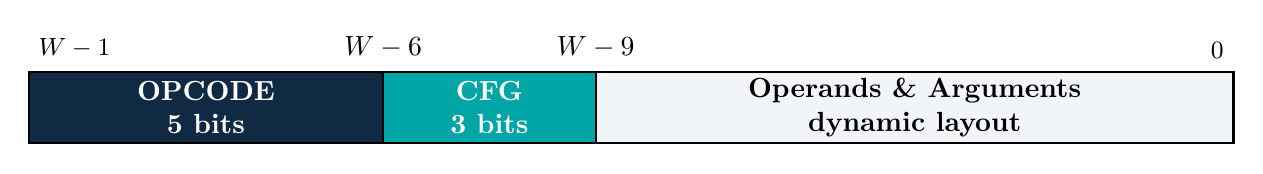
\begin{tikzpicture}[x=0.9cm,y=0.72cm]
  \draw[thick,fill=limblue] (0,0) rectangle (5,1.25);
  \draw[thick,fill=limcyan] (5,0) rectangle (8,1.25);
  \draw[thick,fill=limlight] (8,0) rectangle (17,1.25);
  \node[text=white,font=\bfseries,align=center] at (2.5,0.62) {OPCODE\\5 bits};
  \node[text=white,font=\bfseries,align=center] at (6.5,0.62) {CFG\\3 bits};
  \node[font=\bfseries,align=center] at (12.5,0.62) {Operands \& Arguments\\dynamic layout};
  \node[anchor=south west,font=\small] at (0,1.32) {$W-1$};
  \node[anchor=south] at (5,1.32) {$W-6$};
  \node[anchor=south] at (8,1.32) {$W-9$};
  \node[anchor=south east,font=\small] at (17,1.32) {0};
\end{tikzpicture}
\end{center}

The 3-bit \field{cfg} field selects up to 8 orthogonal execution modes per opcode, enabling expressive addressing and operand variations without opcode proliferation.

\section{Instruction Set Architecture Summary}
\small
\begin{longtable}{r>{\ttfamily}p{13mm}>{\ttfamily}p{19mm}p{28mm}p{75mm}}
\toprule
No. & Code & Mnemonic & Class & Functional Summary \\
\midrule\endhead
0  & 00000 & NOP  & Control     & No operation and ALU residual chain flush \\
1  & 00001 & ADD  & Arithmetic  & Addition with automatic multi-word carry chaining \\
2  & 00010 & SUB  & Arithmetic  & Subtraction with automatic multi-word borrow chaining \\
3  & 00011 & MUL  & Arithmetic  & Integer multiplication with upper word residual latching \\
4  & 00100 & DIV  & Arithmetic  & Integer division with remainder latched in ALU residual \\
5  & 00101 & LMR  & Memory      & Load memory word into register \\
6  & 00110 & LRM  & Memory      & Store register word into memory \\
7  & 00111 & LRR  & Transfer    & Low-latency register-to-register copy via bypass MUX \\
8  & 01000 & CMP  & Compare     & Arithmetic compare without modifying operand registers \\
9  & 01001 & JMP  & Branch      & Unconditional branch (direct, indirect, 24-bit pointer) \\
10 & 01010 & JCR  & Branch      & Conditional branch on Carry Flag (CF) \\
11 & 01011 & JNZ  & Branch      & Conditional branch on Non-Zero (ZF = 0) \\
12 & 01100 & JZ   & Branch      & Conditional branch on Zero (ZF = 1) \\
13 & 01101 & AND  & Logic       & Bitwise logical AND \\
14 & 01110 & OR   & Logic       & Bitwise logical OR \\
15 & 01111 & NAND & Logic       & Bitwise logical NAND \\
16 & 10000 & NOR  & Logic       & Bitwise logical NOR \\
17 & 10001 & NOT  & Logic       & Bitwise bit inversion (one's complement) \\
18 & 10010 & XOR  & Logic       & Bitwise exclusive OR \\
19 & 10011 & XNOR & Logic       & Bitwise equivalence \\
20 & 10100 & INC  & Arithmetic  & Atomic increment operand by 1 \\
21 & 10101 & DEC  & Arithmetic  & Atomic decrement operand by 1 \\
22 & 10110 & PUSH & Stack       & Push word onto execution stack \\
23 & 10111 & POP  & Stack       & Pop word from execution stack into destination \\
24 & 11000 & BSL  & Shift       & Barrel shift left with configurable fill \\
25 & 11001 & BSR  & Shift       & Barrel shift right with discarded bit capture \\
26 & 11010 & CSRM & System      & Privileged control and status register access \\
27 & 11011 & RSV27 & Reserved   & Reserved for vector/SIMD processing extensions \\
28 & 11100 & RSV28 & Reserved   & Reserved for extended addressing modes \\
29 & 11101 & RSV29 & Reserved   & Reserved for floating-point coprocessor \\
30 & 11110 & RSV30 & Reserved   & Reserved for hardware cryptographic acceleration \\
31 & 11111 & RSV31 & Reserved   & Reserved for future architectural expansion \\
\bottomrule
\end{longtable}
\normalsize

\section{Detailed Instruction Specifications}
The following pages detail the formal execution profiles for all 32 opcode allocations.

\InstructionPage{NOP}{00000}{Control}{No Operation and Arithmetic Chain Flush}{%
PC <- PC + instruction\_length \\
ALU\_RESIDUAL <- 0 \\
FREG.CF <- 0 \\
FREG.OF <- 0%
}{No operands required; \field{cfg} field reserved for delay calibration.}{Clears carry (CF), overflow (OF), and borrow tracking flags; preserves other flags.}{Performs pipeline cycle alignment and flushes the internal ALU residual accumulator, terminating any chained multi-word carry/borrow sequence before starting new independent calculations.}
\InstructionPage{ADD}{00001}{Arithmetic}{Addition with Automatic Multi-Word Carry Chaining}{%
sum\_full <- srcA + srcB + ALU\_RESIDUAL \\
dst <- sum\_full[15:0] \\
ALU\_RESIDUAL <- (sum\_full > 0xFFFF ? 1 : 0)%
}{GPRs R0--R7, accumulators ACCA/ACCB, or immediate operands.}{Sets carry flag CF and overflow OF if sum exceeds $2^{16}-1$; updates ZF based on dst.}{Delivers seamless multi-word arithmetic (32, 48, 64+ bits). If the addition exceeds 16 bits ($>2^{16}-1$), the carry (+1) is latched into the internal ALU residual register and automatically added during the subsequent ADD operation without requiring distinct ADC opcodes. The lower 16 bits are deterministically stored in dst. The chain is reset via NOP or overwritten by a new operation.}
\InstructionPage{SUB}{00010}{Arithmetic}{Subtraction with Automatic Multi-Word Borrow Chaining}{%
diff\_full <- srcA - srcB - ALU\_RESIDUAL \\
dst <- diff\_full[15:0] \\
ALU\_RESIDUAL <- (diff\_full < 0 ? 1 : 0)%
}{GPRs R0--R7, constants, or accumulators ACCA/ACCB.}{Sets borrow flag (CF) and OF on negative result ($< 0$); updates ZF.}{Enables continuous multi-word subtraction. When a borrow occurs ($< 0$), the borrow ($-1$) is retained in the internal ALU register and automatically subtracted during the next SUB operation. The lower 16-bit word is deterministically preserved in dst. Inserting a NOP breaks the chain for independent subtraction.}
\InstructionPage{MUL}{00011}{Arithmetic}{Multiplication with Upper Word Residual Retention}{%
prod <- srcA * srcB \\
dst <- prod[15:0] \\
ALU\_RESIDUAL <- prod[31:16]%
}{GPRs R0--R7, accumulators ACCA/ACCB.}{Updates ZF; sets OF/CF if the upper 16 bits of the product (prod[31:16]) are non-zero.}{For 32-bit products exceeding the 16-bit register width, the low 16 bits are placed into dst, while the upper 16 bits are retained in the internal ALU residual register. In a subsequent addition, this residual is automatically accumulated (hardware MAC support / bigint multiplication). The upper word can also be extracted by adding the register to itself after clearing. Executing NOP flushes the residual register.}
\InstructionPage{DIV}{00100}{Arithmetic}{Division with Remainder Latched in ALU Residual}{%
dst <- srcA / srcB \\
ALU\_RESIDUAL <- srcA \% srcB%
}{GPRs R0--R7, accumulators ACCA/ACCB.}{Sets EM (Error Math) flag on division by zero without core stall; updates ZF.}{Stores the integer quotient in dst while preserving the remainder (modulo) in the internal ALU residual register for immediate reuse in subsequent operations or clearing via NOP.}
\InstructionPage{LMR}{00101}{Memory}{Load Word from Memory to Register}{dst\_reg <- MEM[address]}{Addressing: direct, indirect via \reg{PTREG}, or base-plus-offset.}{Preserves all status flags.}{Supports automated hardware pointer increment when AIP is set.}
\InstructionPage{LRM}{00110}{Memory}{Store Register Word to Memory}{MEM[address] <- src\_reg}{Addressing mode configured via \field{cfg} and pointer register \reg{PTREG}.}{Preserves all status flags.}{Direct transfer from register file to memory bus without intermediate staging.}
\InstructionPage{LRR}{00111}{Transfer}{Low-Latency Register-to-Register Copy}{dst\_reg <- src\_reg}{Arguments specify source and destination registers.}{Preserves all status flags.}{Routes via the dedicated MUX 1 $\to$ MUX 2 bypass, leaving the ALU unblocked.}
\InstructionPage{CMP}{01000}{Compare}{Hardware Operand Comparison}{FREG.CMP <- compare(srcA, srcB)}{Register or immediate comparison modes.}{Updates 2-bit FREG.CMP field and flags ZF, CF, OF without modifying registers.}{Enables swift condition evaluation without data corruption.}
\InstructionPage{JMP}{01001}{Branch}{Unconditional Program Branch}{PC <- target}{Supports 16-bit relative, direct absolute, or full 24-bit jump via \reg{PTREG}.}{Preserves all status flags.}{Atomic reload of the Program Counter in minimal clock cycles.}
\InstructionPage{JCR}{01010}{Branch}{Conditional Branch on Carry}{if FREG.CF == 1 then PC <- target}{Target specified via relative displacement or absolute address.}{Flags read without modification.}{Foundational primitive for multi-word extended precision arithmetic loops.}
\InstructionPage{JNZ}{01011}{Branch}{Conditional Branch on Non-Zero}{if FREG.ZF == 0 then PC <- target}{High-efficiency branch for loop counters and iterative structures.}{Preserves all status flags.}{Fast-path condition evaluation in microcode.}
\InstructionPage{JZ}{01100}{Branch}{Conditional Branch on Zero}{if FREG.ZF == 1 then PC <- target}{Evaluates termination or equality conditions.}{Preserves all status flags.}{Optimized for string matching and search algorithms.}
\InstructionPage{AND}{01101}{Logic}{Bitwise Logical AND}{dst <- srcA AND srcB}{Register operands or immediate bitmasks.}{Updates Zero Flag (ZF); resets overflow status.}{Essential for bitmask extraction and masking.}
\InstructionPage{OR}{01110}{Logic}{Bitwise Logical OR}{dst <- srcA OR srcB}{Register operands or bitfield insertion.}{Updates ZF; carry/overflow deterministically cleared.}{Rapid combination of control bitfields.}
\InstructionPage{NAND}{01111}{Logic}{Bitwise Logical NAND}{dst <- NOT (srcA AND srcB)}{Universal logic primitive.}{Updates ZF.}{Enables compact implementation of custom Boolean functions.}
\InstructionPage{NOR}{10000}{Logic}{Bitwise Logical NOR}{dst <- NOT (srcA OR srcB)}{Inverted logic primitive.}{Updates ZF.}{Broadens fast bitwise logic transformations.}
\InstructionPage{NOT}{10001}{Logic}{Bitwise Inversion (One's Complement)}{dst <- NOT src}{High-speed unary inversion.}{Updates ZF.}{Executes in minimal microcycles.}
\InstructionPage{XOR}{10010}{Logic}{Bitwise Exclusive OR}{dst <- srcA XOR srcB}{Used for bit flipping and rapid register zeroing.}{Updates ZF.}{Foundational for parity, CRC, and cryptographic ciphers.}
\InstructionPage{XNOR}{10011}{Logic}{Bitwise Equivalence}{dst <- NOT (srcA XOR srcB)}{Bit-by-bit identity testing.}{Updates ZF.}{Fast parallel mask equivalence validation.}
\InstructionPage{INC}{10100}{Arithmetic}{Atomic Increment by 1}{dst <- src + 1}{Fast loop iterator step.}{Updates ZF, OF; Carry Flag preserved or updated based on \field{cfg}.}{Optimizes array index advancing.}
\InstructionPage{DEC}{10101}{Arithmetic}{Atomic Decrement by 1}{dst <- src - 1}{Fast downward counter step.}{Updates ZF, OF.}{Compact loop termination construct.}
\InstructionPage{PUSH}{10110}{Stack}{Push Word onto Execution Stack}{%
stack <- src \\
SREG <- SREG - 2%
}{Source: any GPR (R0--R7) or special status register.}{Preserves arithmetic flags.}{Hardware-assisted subroutine and context preservation.}
\InstructionPage{POP}{10111}{Stack}{Pop Word from Execution Stack}{%
dst <- stack \\
SREG <- SREG + 2%
}{Destination: any GPR or status register.}{Preserves arithmetic flags.}{Symmetric restoration of execution contexts.}
\InstructionPage{BSL}{11000}{Shift}{Barrel Shift Left}{dst <- src << amount}{Shift count: immediate constant or dynamic register value.}{Ejected MSB latched into FREG.DBIT; supports SMOD/SBIT insertion.}{High-speed arithmetic scaling and bitfield alignment.}
\InstructionPage{BSR}{11001}{Shift}{Barrel Shift Right}{dst <- src >> amount}{Logical or sign-extended arithmetic right shift selectable via \field{cfg}.}{Discarded LSB latched into FREG.DBIT.}{Fast scaling and power-of-two division.}
\InstructionPage{CSRM}{11010}{System}{Control and Status Register Access}{special\_reg <- src OR dst <- special\_reg}{Access to \reg{FREG}, \reg{PTREG}, and \reg{SREG}.}{Flags updated when FREG is modified.}{Privileged context switching and configuration primitive.}
\InstructionPage{RSV27}{11011}{Reserved}{Architectural Extension Slot}{reserved}{Reserved for future LIM ISA revisions.}{Undefined.}{Reserved.}
\InstructionPage{RSV28}{11100}{Reserved}{Architectural Extension Slot}{reserved}{Reserved for future LIM ISA revisions.}{Undefined.}{Reserved.}
\InstructionPage{RSV29}{11101}{Reserved}{Architectural Extension Slot}{reserved}{Reserved for future LIM ISA revisions.}{Undefined.}{Reserved.}
\InstructionPage{RSV30}{11110}{Reserved}{Architectural Extension Slot}{reserved}{Reserved for future LIM ISA revisions.}{Undefined.}{Reserved.}
\InstructionPage{RSV31}{11111}{Reserved}{Architectural Extension Slot}{reserved}{Reserved for future LIM ISA revisions.}{Undefined.}{Reserved.}

\clearpage
\section{Physical Package and Pinout (34-Pin Form Factor)}
The processor is packaged in a high-reliability dual-inline 34-pin enclosure:

\begin{center}
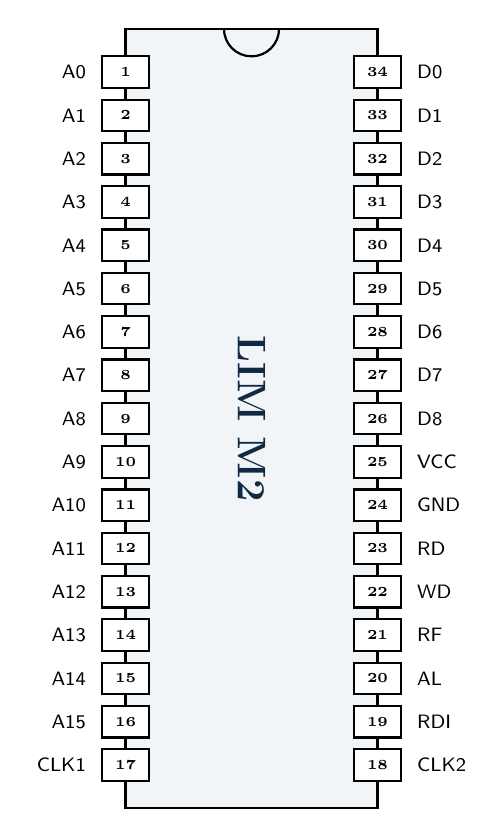
\begin{tikzpicture}[font=\sffamily\scriptsize,
  pinbox/.style={draw,thick,fill=white,minimum width=6mm,minimum height=4mm,inner sep=0pt,font=\bfseries\tiny}]
\def\chipW{3.2}
\def\chipH{9.9}
\draw[thick,fill=limlight] (0,0) rectangle (\chipW,-\chipH);
\draw[thick] ($(\chipW/2,0)+(-0.35,0)$) arc (180:360:0.35);
\node[font=\bfseries\Large,text=limblue,rotate=-90] at (\chipW/2,-\chipH/2) {LIM M2};
\foreach \i/\sigL/\sigR in {
  1/A0/D0, 2/A1/D1, 3/A2/D2, 4/A3/D3, 5/A4/D4, 6/A5/D5, 7/A6/D6, 8/A7/D7,
  9/A8/D8, 10/A9/VCC, 11/A10/GND, 12/A11/RD, 13/A12/WD, 14/A13/RF, 15/A14/AL, 16/A15/RDI, 17/CLK1/CLK2
} {
  \pgfmathsetmacro{\y}{-\i * 0.55}
  \pgfmathtruncatemacro{\pinR}{35 - \i}
  \node[pinbox] at (0,\y) {\i};
  \node[anchor=east] at (-0.38,\y) {\sigL};
  \node[pinbox] at (\chipW,\y) {\pinR};
  \node[anchor=west] at (\chipW+0.38,\y) {\sigR};
}
\end{tikzpicture}
\end{center}

\subsection{Pin Descriptions}
\begin{tabularx}{\textwidth}{>{\ttfamily}p{28mm}p{24mm}X}
\toprule
Signal & Direction & Functional Role \\
\midrule
A0--A15    & Output / Tri-State & 16-bit primary address bus (latched via external AL strobe). \\
D0--D7     & Bidirectional      & 8-bit external memory and peripheral data interface. \\
CLK1, CLK2 & Input              & Two-phase non-overlapping clock synchronization inputs. \\
VCC, GND   & Power              & Primary power supply rails (+5 V nominal). \\
RD, WD     & Output             & Bus Read Enable and Write Enable strobes. \\
AL         & Output             & Address Latch strobe for external high-speed address registers. \\
RF         & Input              & Ready Flag: external slave memory handshake acknowledge. \\
RDI        & Input              & Raw Direct Interrupt: priority hardware interrupt request line. \\
\bottomrule
\end{tabularx}

\section{Conclusion}
The \textbf{LIM M2} architecture harmonizes the time-tested reliability of deterministic microprogramming with the modern performance of an entirely tri-state-free multiplexer datapath. By eliminating bus contention, floating nodes, and capacitive decay, the LIM M2 guarantees exceptional signal fidelity and opens an unprecedented clock frequency envelope spanning from 200~MHz to the highest thresholds of modern silicon.
\end{document}
